% !TEX TS-program = pdflatex
% !TEX encoding = UTF-8 Unicode

\documentclass[11pt]{article} % use larger type; default would be 10pt

\usepackage[utf8]{inputenc} % set input encoding (not needed with XeLaTeX)
\usepackage{graphicx} % support the \includegraphics command and options
\usepackage[parfill]{parskip} % Activate to begin paragraphs with an empty line rather than an indent
\usepackage{verbatim} % adds environment for commenting out blocks of text & for better verbatim
\usepackage[hidelinks]{hyperref}
\usepackage{caption}
\usepackage{subcaption}

\title{jClustering v1.3.0 user manual}
\author{José María Mateos \\ \texttt{jmmateos@mce.hggm.es}}

\begin{document}
\maketitle

\tableofcontents

\section{Introduction}

jClustering is an ImageJ plugin for dynamic (3D + time or 2D + time) segmentation. It groups
image voxels by similarity of their temporal behavior. This is a brief user manual that explains
how to use jClustering within a working ImageJ installation.

For further information regarding jClustering, please refer to the published paper (see section \ref{sec:reference}).

This manual refers to jClustering v1.3.0 and beyond. It will not be edited just to update this version number. Unless
there are significative changes in a new version, do not expect this number to match the latest release.

\section{Download and installation}

The installation procedure is straightforward, you just need to follow these steps:

\begin{enumerate}
\item Download the latest jClustering release from \url{https://github.com/HGGM-LIM/jclustering/releases} and copy the 
\texttt{jClustering\_.jar} file into the \texttt{plugins/} directory of your ImageJ installation.

\item Download the latest Apache Commons Math library from \url{http://commons.apache.org/math/download_math.cgi}
(it should be a file with a name in the form of \texttt{commons-math3-3.X-bin.zip}, where X is the most recent version number,
open it with any unzip program and copy the file \texttt{commons-math3-3.X/commons-math3-3.X.jar} to the 
\texttt{plugins/jars} directory of your ImageJ installation.

\item Same for the fastICA library. Go to its webpage (\url{http://sourceforge.net/projects/fastica/}) and store the .jar file
in the \texttt{plugins/jars} directory of your ImageJ installation.
\end{enumerate}

jClustering has been tested on ImageJ versions newer than 1.46r (included) and JRE 6.

\section{Main window}

When you run jClustering (Plugins $>$ Clustering $>$ jClustering) with an ImageJ hyperstack open, you will get the main
window (figure \ref{fig:main}).

\begin{figure}[h!]
  \centering
    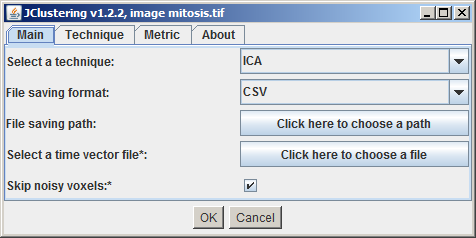
\includegraphics[width=\textwidth]{figures/main_window}
  \caption{Main jClustering window.}
  \label{fig:main}
\end{figure}

If a hyperstack is not present, an error dialog will pop-up. jClustering works on images that have already been opened and
displays the name of the image it is acting upon on the main window title bar. If you wish to run clustering operations on
another image, select it and run another instance of jClustering.

The different options are:

\begin{itemize}
\item {\em Select a technique:} select a clustering technique. Please refer for the next sections for information on each one
of them.
\item {\em File saving format:} choose the format in which the text files containing the time-activity curves for each cluster
will be stored. Current values are CSV (comma-separated values), PMOD (for the PMOD software, \url{http://www.pmod.com})
and tab-separated.
\item {\em File saving path:} if you specify a path here, the text file will be saved in that path. The name of the text file
begins with \texttt{jclustering} and includes a timestamp of the time of the analysis.
\item {\em Select a time vector file:} ImageJ does not read different frame length information from the image header. If you
want the frame start and end times to appear in your results text file, you need to specify it here. The format of this file is a
space or tab-separated file with two columns: frame start and frame end time. For instance:

\begin{verbatim}
0.0	2.0
2.0	4.0
4.0	6.0
...
\end{verbatim}

\end{itemize}

\section{Implemented clustering techniques}

The options for the different clustering techniques implemented in jClustering are shown below.

\subsection{Independent Component Analysis (ICA)}

The ICA technique tab is shown in figure \ref{fig:ica_window}.

\begin{figure}[h!]
  \centering
    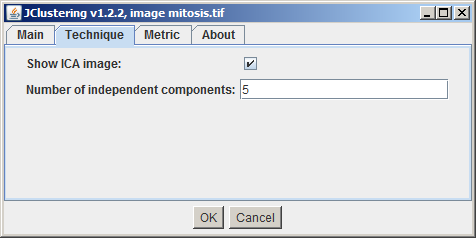
\includegraphics[width=\textwidth]{figures/ica_window}
  \caption{Independent Component Analysis window.}
  \label{fig:ica_window}
\end{figure}

The different options are:

\begin{itemize}
\item {\em Show ICA image:} as jClustering shows the final clustering result based on a \emph{winner-takes-it-all} approach,
it may be useful to show on screen the resulting ICA analysis. This image will show up if this option is checked (it is by default).

\item {\em Number of independent components:} the estimated number of independent components. Defaults to 5.

\end{itemize}

This clustering technique also outputs the independent components found on the output directory, if this has been chosen.

\subsection{K-means}

The k-means technique tab is shown in figure \ref{fig:k-means_window}.

\begin{figure}[h!]
  \centering
    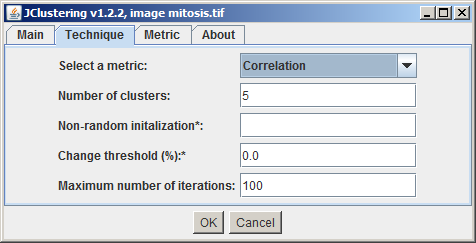
\includegraphics[width=\textwidth]{figures/k-means_window}
  \caption{K-means window.}
  \label{fig:k-means_window}
\end{figure}

The different options are:
\begin{itemize}
\item {\em Select a metric:} selects one of the implemented metrics. Please refer to section \ref{sec:metrics} for more
information.
\item {\em Number of clusters:} the initial number of clusters to create. Defaults to 5. The final result may yield fewer clusters, as
some might be emptied during the iterative process.
\item {\em Non-random initialization:} if you wish to select all or some initial centroids you can write the coordinates here
with the following format: \texttt{x1,y1,z1;x2,y2,z2}, where x, y and z are the 3D coordinates of the centroid. If you define
fewer points than the configured number of clusters, the rest will be randomly chosen. If you write \texttt{++} here, a 
k-means++ initialization algorithm will be used. Use \texttt{det++} for a \emph{deterministic} k-means initialization, in which 
the first centroid corresponds to the time-activity curve with the highest maximum amplitude.
\item {\em Change threshold (\%):} the amount of change allowed between clusters to end the iterative process. By default,
all clusters must remain the same between two given iterations to stop.
\item {\em Maximum number of iterations:} the maximum number of iterations allowed. If no convergence is achieved and this
number of iterations is reached, the program finishes with the clusters currently in memory.

\end{itemize}

\subsection{Leader-follower}

The leader-follower technique tab is shown in figure \ref{fig:leader-follower_window}.

\begin{figure}[h!]
  \centering
    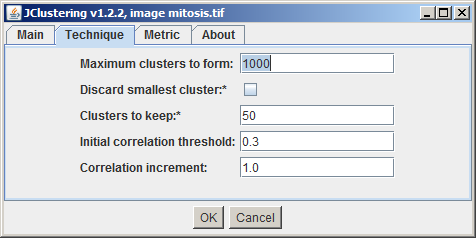
\includegraphics[width=\textwidth]{figures/leader-follower_window}
  \caption{Leader-follower window.}
  \label{fig:leader-follower_window}
\end{figure}

The different options are:

\begin{itemize}
\item {\em Maximum clusters to form:} the maximum number of clusters the algorithm will create.
\item {\em Discard smallest cluster:} if the maximum number of clusters is reached and a new one needs to be created,
the smallest one (the one with fewer voxels and lower mean amplitude) is discarded and a new one is created when this
box is checked. When unchecked, voxels that need to create a new cluster are discarded.
\item {\em Clusters to keep:} the number of clusters that will be shown on screen when the algorithm finishes. As it normally
creates a great number of clusters, it is better to keep this number low. Clusters are shown on screen ordered by the number
of voxels they contain, with the biggest ones first.
\item {\em Initial correlation threshold:} the initial correlation threshold use to create new clusters.
\item {\em Correlation increment:} a multiplicative variable that increments the correlation threshold of a given cluster. When
set to a value greater than $1.0$, the correlation threshold for a given cluster is incremented every time a new voxel is added.
No increment is set by default.
 
\end{itemize}

\subsection{Principal Component Analysis (PCA)}

The PCA technique tab is shown in figure \ref{fig:pca_window}.

\begin{figure}[h!]
  \centering
    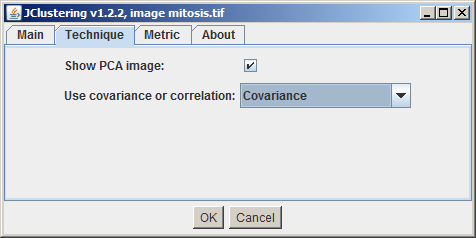
\includegraphics[width=\textwidth]{figures/pca_window}
  \caption{PCA window.}
  \label{fig:pca_window}
\end{figure}

The different options are:

\begin{itemize}
\item {\em Show PCA image:} same as the ICA case. If you wish to visualize the final PCA result, check this box.
\item {\em Use covariance or correlation:} PCA is computed by applying SVD to the covariance matrix. In some cases, the
correlation matrix may also be used. This dialog allows you to select either one. Defaults to covariance.
\end{itemize}

This clustering technique also writes to file the values of the principal components.

\subsection{Singular Value Decomposition (SVD)}

The SVD technique tab is shown in figure \ref{fig:svd_window}.

\begin{figure}[h!]
  \centering
    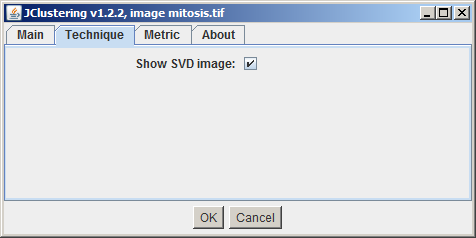
\includegraphics[width=\textwidth]{figures/svd_window}
  \caption{SVD window.}
  \label{fig:svd_window}
\end{figure}

The only option is to show the SVD image, as in the ICA and PCA cases. SVD computation is done by applying SVD to the
whole image matrix, not to the correlation or covariance one (PCA).

This clustering technique also writes to file the values of the eigenvectors found.

\section{Implemented metrics (distances)}
\label{sec:metrics}

The different metrics are currently used only the the k-means clustering technique. For more information on the 
particular metrics implemented, please refer to the original jClustering paper on PLOS ONE.

\section{Results presentation and interpretation}
\label{sec:results}

This section details how jClustering shows the results on screen and how they should be interpreted. The reader will also
find here details on how the text files are stored.

\subsection{Graphical display}
\label{subsec:results_graphical}

jClustering shows the resulting segmentation clusters in a new 4D image. This image has $n+1$ frames, with $n$ being the
total number of clusters formed. Each frame of this image represents each individual cluster, with the voxels belonging to it
with a non-zero value. The last frame is useful for visualizing all clusters at the same time; in this representation, each one is 
displayed with a different grayscale value.

In figure \ref{fig:results_example} the results from a 5 clusters k-means are shown.

\begin{figure}
        \centering
        \begin{subfigure}[b]{0.3\textwidth}
                \centering
                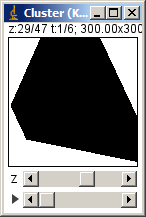
\includegraphics[width=\textwidth]{figures/k-means_results_1}
                \caption{First cluster}
                \label{fig:k-means_res_1}
	\end{subfigure}%
	 ~
        \begin{subfigure}[b]{0.3\textwidth}
                \centering
                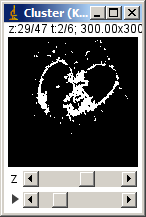
\includegraphics[width=\textwidth]{figures/k-means_results_2}
                \caption{Second cluster}
                \label{fig:k-means_res_2}
	\end{subfigure}%
	 ~
        \begin{subfigure}[b]{0.3\textwidth}
                \centering
                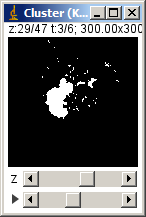
\includegraphics[width=\textwidth]{figures/k-means_results_3}
                \caption{Third cluster}
                \label{fig:k-means_res_3}
	\end{subfigure}%
	 \\
        \begin{subfigure}[b]{0.3\textwidth}
                \centering
                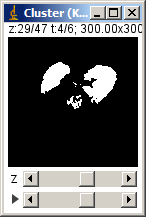
\includegraphics[width=\textwidth]{figures/k-means_results_4}
                \caption{Fourth cluster}
                \label{fig:k-means_res_4}
	\end{subfigure}%
	 ~
        \begin{subfigure}[b]{0.3\textwidth}
                \centering
                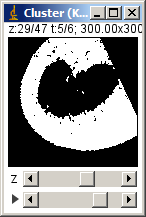
\includegraphics[width=\textwidth]{figures/k-means_results_5}
                \caption{Fifth cluster}
                \label{fig:k-means_res_5}
	\end{subfigure}%
	 ~
        \begin{subfigure}[b]{0.3\textwidth}
                \centering
                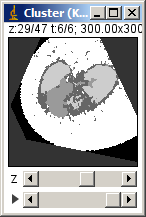
\includegraphics[width=\textwidth]{figures/k-means_results_6}
                \caption{All clusters at once}
                \label{fig:k-means_res_6}
	\end{subfigure}%
	 \caption{Example of final clustering displaying by jClustering using ImageJ's HyperStacks}\label{fig:results_example}
\end{figure}

It is important to note that this convention is used then {\em deterministic} clusters are used. Some techniques, such as PCA,
also have the possibility of displaying the computed principal components. These techniques (currently: ICA, PCA and SVD) 
generate their clusters by using a winner-takes-it-all approach, in which the independent component / principal component or
singular value with the greatest value is used to assign each voxel. In any case, the mathematical representation of the images
may be useful if the user wishes to do some more elaborated processing. For instance, when the PCA cluster is set to show
the PCA image, the same approach is used: a HyperStack is returned (in addition to the original clusters) and each principal
component is shown in a different frame.

\subsection{Text files}
\label{subsec:results_text}

More important than the visual representation of the formed clusters are the values of the time-activity curves of the different
clusters. These values will be stored to a file if the {\em File saving path} option has been set in the main tab; the TAC for
each cluster will be stored as a column in that file, every frame is a row.

The format for this file must be chosen by the user through the {\em File saving format} option and also depends on whether
a time file vector with the frame starting and end times has been specified. If this has been the case, the first two columns
are taken from that vector file. In the case of the PMOD format, as the frame information is mandatory, if no time vector file
has been provided, hard-coded frame information (each frame lasting 1 second) will be used. This is hardly optimal and will yield incorrect kinetic parameters if used in this form, but that is what that specific format requires. The user must correct these values before using is an input for any posterior analysis.

\section{Reference}
\label{sec:reference}

Mateos-Pérez JM, García-Villalba C, Pascau J, Desco M, Vaquero JJ (2013) jClustering, an Open Framework for the Development of 4D Clustering Algorithms. PLoS ONE 8(8): e70797. doi:10.1371/journal.pone.0070797. Available at
\url{http://www.plosone.org/article/info\%3Adoi\%2F10.1371\%2Fjournal.pone.0070797}.

\end{document}
